\chapter{Introduction about NALCO}

National Aluminium Company Limited (NALCO) is one of the leading public sector enterprises in India engaged in the production of alumina and aluminium. Established in the year 1981, NALCO operates under the Ministry of Mines, Government of India, and is recognized as one of the largest integrated Bauxite-Alumina-Aluminium-Power complexes in the country. The company plays a major role in India’s aluminium industry through its mining, refining, smelting, and power generation operations.

As a globally recognized Navratna Central Public Sector Enterprise (CPSE), NALCO is renowned for its operational excellence and financial performance. Its integrated complex manages every stage of production from raw material extraction to the final product. The strategic planning and corporate governance that drive this vast operation originate from its central headquarters in Bhubaneswar.

\begin{figure}[!ht]
    \centering
    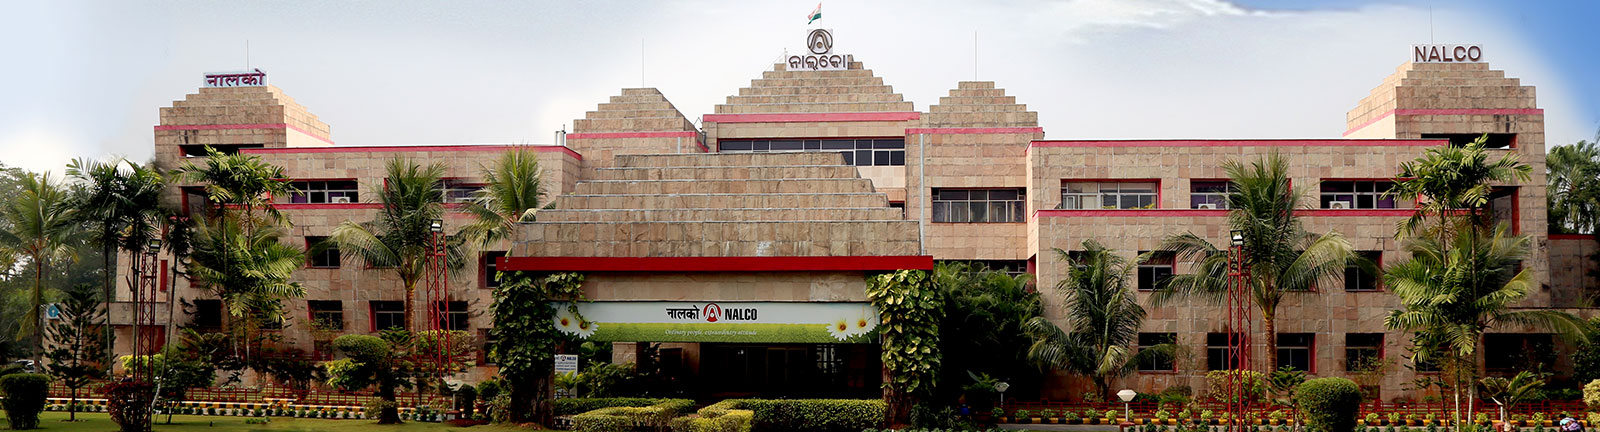
\includegraphics[width=1.0\textwidth]{nalco-corporate office.jpg}
    \caption{NALCO's Corporate Office in Bhubaneswar, serving as the administrative nerve center.}
    \label{fig:corporate}
\end{figure}

The distinct architectural form of NALCO's corporate office building serves as the administrative nerve center. This structure reflects the company's strong industrial presence and oversees the entire spectrum of its diverse operations across multiple locations, ensuring NALCO's position as a globally competitive enterprise and its sustained contribution to India's industrial growth.

\FloatBarrier
\section{Panchpatmali Bauxite Mines}

The first vital link in NALCO's integrated chain is the extraction of raw material. NALCO operates the Panchpatmali Bauxite Mines, located near Damanjodi, which serve as the primary source of bauxite ore. These mines are highly mechanized and rank among the largest open-cast bauxite mines in Asia. The mining operations follow modern techniques and rigorous environmental conservation measures to ensure sustainable practices.

\begin{figure}[!ht]
    \centering
    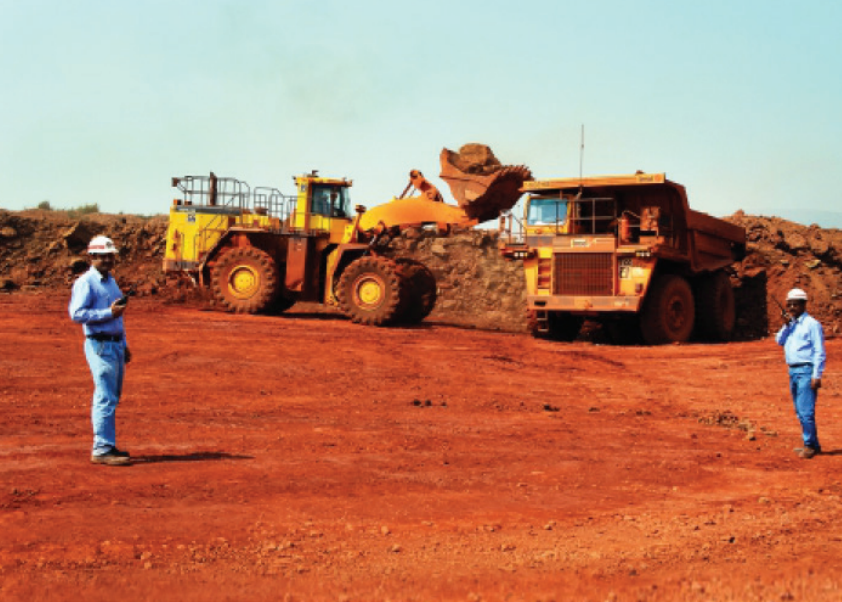
\includegraphics[width=0.8\textwidth]{Chapters/bauxitemine.png}
    \caption{Heavy machinery operating at the Panchpatmali Bauxite Mines.}
    \label{fig:mines}
\end{figure}

The continuous and efficient operation of these mines relies heavily on advanced heavy earth-moving machinery. The scale of this mechanized extraction is clearly visible in the rich, red terrain of the mine. Personnel oversee massive front-end loaders and heavy-duty dump trucks working systematically to extract and load the bauxite ore for transport.

\FloatBarrier
\section{NALCO Alumina Refinery, Damanjodi}

Following the initial mining process, the bauxite ore is transported to the Alumina Refinery located at Damanjodi in the Koraput district of Odisha. This refinery processes the bauxite ore into alumina through the specialized Bayer Process, serving as a critical bridge in NALCO's value chain.

\begin{figure}[!ht]
    \centering
    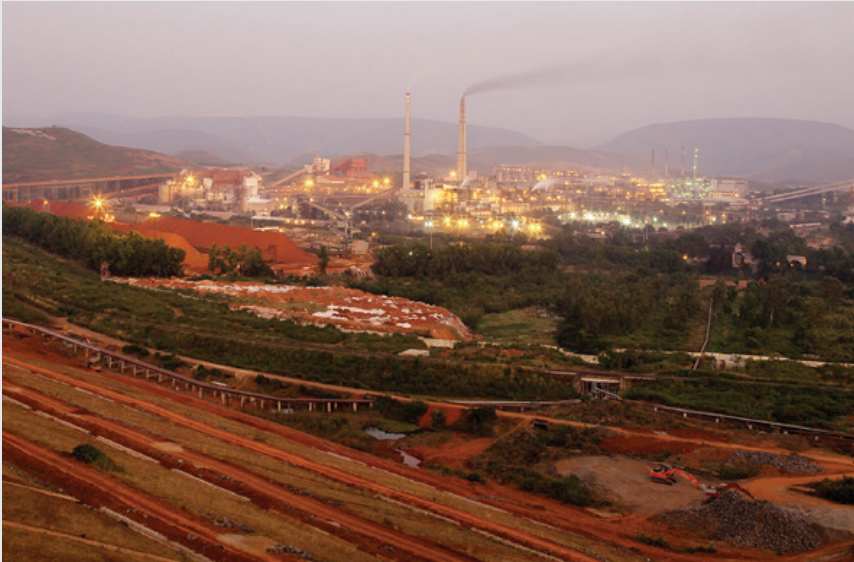
\includegraphics[width=0.8\textwidth]{Chapters/aluminarefinary.png}
    \caption{Dusk view of the sprawling NALCO Alumina Refinery at Damanjodi.}
    \label{fig:refinery}
\end{figure}

The Damanjodi refinery is equipped with advanced process control systems, extensive bauxite handling facilities, and vast chemical processing units, including multiple calcination kilns. The sprawling nature of this refinery, nestled against a backdrop of rolling hills, is captured dramatically at dusk with its extensive network of illuminated processing plants and operational smokestacks.

\FloatBarrier
\section{Captive Power Plant}

Aluminium production is an incredibly energy-intensive process, specifically during the smelting stage. To ensure an economical and uninterrupted supply of electricity, NALCO operates a massive dedicated Captive Power Plant. This thermal power facility guarantees the company's energy security and competitive operational independence.

\begin{figure}[!ht]
    \centering
    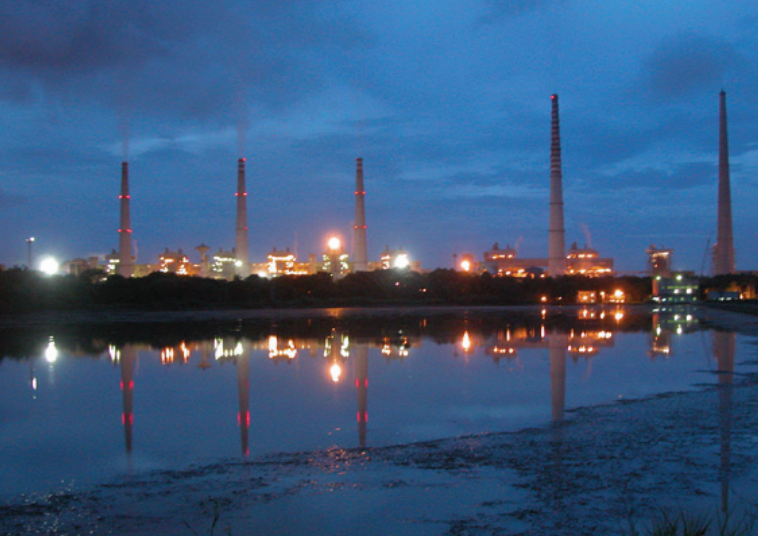
\includegraphics[width=0.8\textwidth]{Chapters/captivepowerplant.png}
    \caption{The illuminated Captive Power Plant ensuring uninterrupted energy supply.}
    \label{fig:powerplant}
\end{figure}

The striking profile of this critical power generation complex is shown brilliantly illuminated against the evening sky. The towering smokestacks and cooling infrastructure of the plant are reflected clearly over the adjacent body of water, illustrating its substantial scale and continuous operation.

\FloatBarrier
\section{Aluminium Smelter Complex}

The pure alumina refined at Damanjodi and the reliable power generated by the captive plant come together at NALCO’s large-scale aluminium smelter. This complex is where the actual production of metal occurs, using an electrolytic process to convert alumina into high-grade molten aluminium, which is then cast into various commercial forms.

\begin{figure}[!ht]
    \centering
    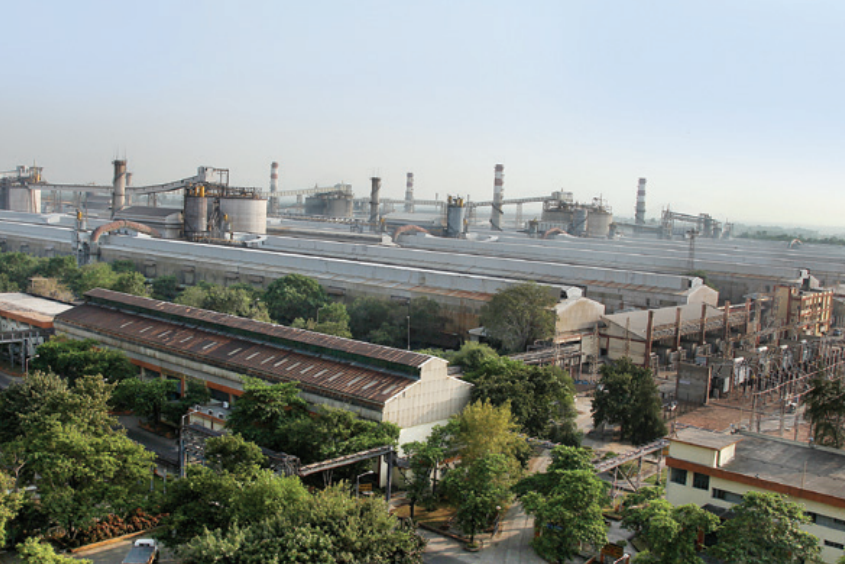
\includegraphics[width=0.8\textwidth]{Chapters/smelter.png}
    \caption{Aerial layout of the massive Aluminium Smelter Complex.}
    \label{fig:smelter}
\end{figure}

The sheer scale and meticulous industrial organization of the smelting facility are highly distinctive. The elevated perspective illustrates the sprawling, grid-like layout of the plant, dominated by exceptionally long, parallel industrial buildings that house the specialized potlines where electrolysis takes place.

\FloatBarrier
\section{Renewable Energy and Sustainability}

Beyond its traditional heavy industrial operations, NALCO is deeply committed to sustainable development and environmental conservation. As a forward-thinking Navratna CPSE, the company actively implements eco-friendly mining practices, waste management systems, extensive afforestation programs, and community development initiatives in its surrounding areas.

\begin{figure}[!ht]
    \centering
    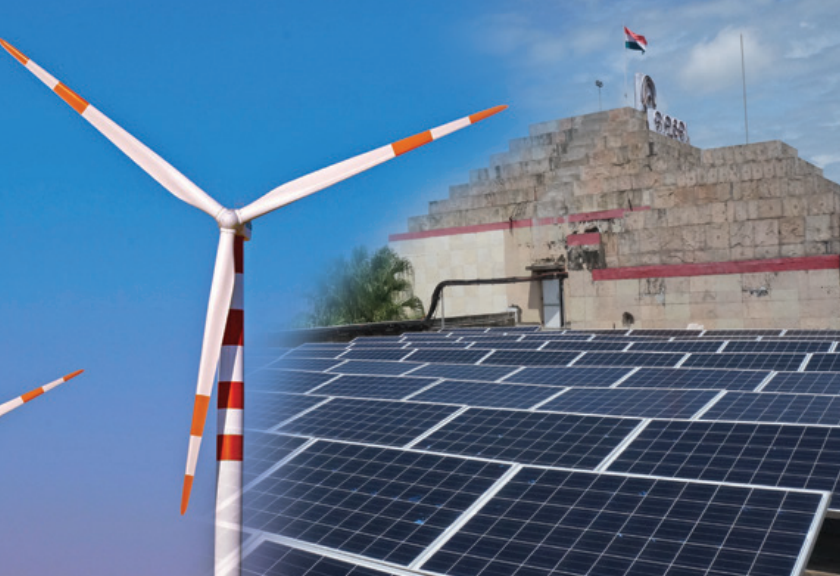
\includegraphics[width=0.8\textwidth]{Chapters/wind_solar.png}
    \caption{NALCO's renewable energy infrastructure including wind turbines and solar panels.}
    \label{fig:renewables}
\end{figure}

Embracing a future of clean energy, NALCO has made significant investments in renewable power sources, adding wind power plants and solar installations to its portfolio. This proactive pivot toward sustainability is visually represented by modern, high-capacity wind turbines working in tandem with a broad array of rooftop solar panels, symbolizing the company's dual commitment to clean industrial energy and traditional operations.

